\documentclass[11pt,a4paper]{article}

% --- Packages ---
\usepackage[utf8]{inputenc}
\usepackage[margin=1in]{geometry}
\usepackage[breaklinks=true,colorlinks,citecolor=blue,linkcolor=blue,urlcolor=blue]{hyperref}
\usepackage[table,xcdraw]{xcolor}
\usepackage{epsfig, mathrsfs, latexsym, subfigure, marginnote, gensymb, amsmath}
\usepackage{graphicx}
\usepackage{booktabs}
\usepackage{adjustbox}
\usepackage{doi}

% Package to handle multiple authors and affiliations cleanly in the article class
\usepackage{authblk} 

% --- Metadata ---
\title{\textbf{pydemi: A Dual-Input Python Framework for Charge-Density-Derived Materials Descriptors via DFT and Machine Learning}}

\author[1]{Shubham Kumar Maurya}
\author[1]{Somnath Bhowmick\thanks{bsomnath@iitk.ac.in}}
\affil[1]{Department of Materials Science \& Engineering, Indian Institute of Technology Kanpur, Kanpur 208016, India}

\date{\today}

% --- Document Start ---
\begin{document}

\maketitle

% --- ABSTRACT -------------------------------------------------------------
\begin{abstract}
The electronic charge density $\rho(\mathbf{r})$ computed by density-functional
theory (DFT) encodes the bonding that materials-property models try to learn,
yet it is rarely used directly as a model input: machine-learning (ML)
featurizers are mostly built on composition and structure, and density-based
analyses such as the quantum theory of atoms in molecules are applied one
structure at a time. We present pydemi, an open-source Python framework that
turns volumetric charge densities into physically interpretable descriptors in
a single batch pipeline. pydemi is organized around one data model and a
periodic geometry pass: derived fields --- the magnetization, an electron
localization function reconstructed from the density, the electrostatic
potential and the deformation density --- are computed once, cached, and
reduced by shared moment, shell-fraction, anisotropy, site-aggregation and
topology operators. The current release computes 220 scalar descriptors in
five domains --- bonding, structural, magnetic, site heterogeneity and,
adopted from matminer, composition --- each registered with its formula,
units, range and documented values for degenerate cases, and each tested for
invariance under supercell expansion, translation and rotation. pydemi reads
densities from VASP and, through cube and XSF files, from other plane-wave
codes, and is designed with a second input path for charge densities
predicted by ML directly from crystal structures.
% TODO: revise the previous sentence once the CIF -> CHGCAR model is integrated.
On a 6,059-structure VASP dataset we quantify how numerical choices affect
the descriptors. Projector-augmented-wave pseudo-densities require dedicated
definitions: 61\% of the densities are negative somewhere, pseudized atoms can
lack a density maximum at the nucleus, 87\% of the deformation density lies
inside the augmentation spheres, and valence counts inferred from electron
configurations disagree with the PAW datasets for 43 of 87 elements. Two
descriptor families are not converged on typical grids: the voxel-averaged
bond ellipticity changes by 20--70\% between derivative schemes, and the
critical-point census closes in only 9\% of the structures, the mismatch being
exactly the number of stencil-dependent extrema. pydemi flags both and
provides a converged, bounded ellipticity. The implementation is validated by
876 automated tests against analytic densities, exact identities and
reference data, and processes the full dataset without failure in 37 CPU
hours.
\end{abstract}

% ==========================================================================
% OUTLINE -- each section lists what it will contain; replace the notes with
% text as the sections are written.
% ==========================================================================

\section{Introduction}
% - Charge density as the fundamental DFT output (Hohenberg-Kohn); why it is
%   an attractive, physically grounded source of ML features.
% - Current practice: composition/structure featurizers (Magpie/matminer),
%   graph networks; density analyses (QTAIM, Bader, critic2) run per
%   structure, not as batch featurizers.
% - Gap: no batch, grid-based, interpretable, numerically controlled
%   density featurizer; ML-predicted densities make such descriptors
%   available without DFT (the dual-input motivation).
% - Contributions: (i) one data model and cached derived fields; (ii) 220
%   descriptors in five domains with a machine-readable registry (formula,
%   units, range, sentinels, stability); (iii) measured numerical and PAW
%   pitfalls and the definitions that avoid them; (iv) validation suite with
%   an invariance harness; (v) dataset application; (vi) open-source release.

\section{Framework design}
\label{sec:framework}

\subsection{Input paths}
pydemi separates reading from featurization: every input is converted into one
data model, and every descriptor is computed from that model only
(Fig.~\ref{fig:architecture}). The first input path reads DFT output. For VASP
it reads \texttt{CHGCAR} files with one (non-spin-polarized), two (collinear)
or four (non-collinear) blocks, the all-electron density
\texttt{AECCAR0}\,+\,\texttt{AECCAR2}, \texttt{ELFCAR} and \texttt{LOCPOT}, and
takes the valence counts (ZVAL) and augmentation radii ($R_{\mathrm{PAW}}$)
from the \texttt{POTCAR} or \texttt{OUTCAR} of the run or from a per-element
table; Gaussian cube and XSF files cover other plane-wave codes. Each density
carries its source (\texttt{pseudo} or \texttt{all\_electron}), which several
definitions depend on (Section~\ref{sec:numerics:paw}). The second input path,
for densities predicted by machine learning from the crystal structure alone,
is described in Section~\ref{sec:ml}.
% TODO: expand once the CIF -> density path is integrated.

\subsection{Data model and numerical core}

\begin{figure}[htbp]
\centering
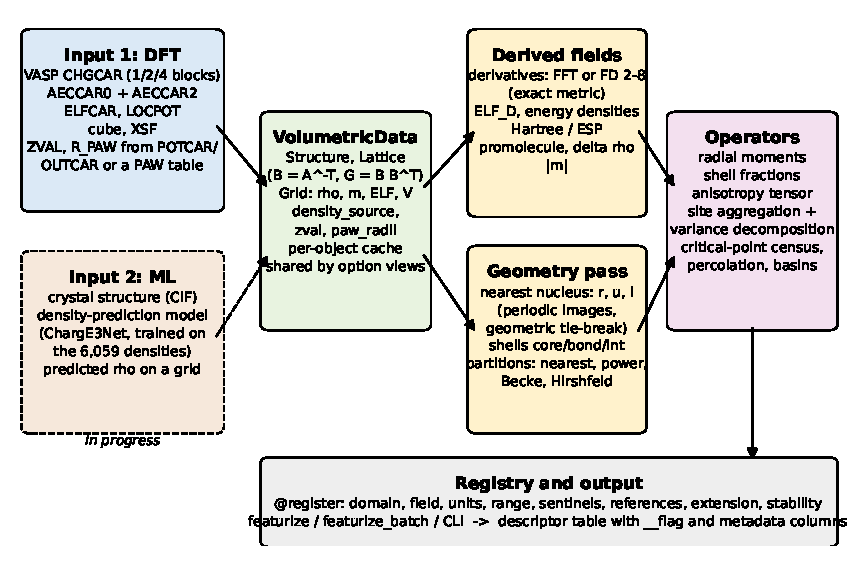
\includegraphics[width=\textwidth]{figures/fig_architecture.pdf}
\caption{Architecture of pydemi. Both input paths produce the same data model;
derived fields and the geometry pass are computed once per structure and
cached, and the operators reduce them to the registered descriptors. The
machine-learning input path (dashed) is being integrated
(Section~\ref{sec:ml}).}
\label{fig:architecture}
\end{figure}

A \texttt{VolumetricData} object holds the structure, the lattice with its
reciprocal basis $B=A^{-\mathsf T}$ and metric $G=BB^{\mathsf T}$, and the
grids of the density $\rho$ (in e\,\AA$^{-3}$), the magnetization, the ELF and
the potential when available. Everything derived from them is cached on the
object, keyed by the options it depends on, so that a descriptor set costs one
evaluation of each field however many descriptors use it, and views of the
same object with other options reuse whatever does not depend on them. The
derived fields are the derivatives of $\rho$ (Section~\ref{sec:numerics:derivatives}),
the electron localization function reconstructed from the density
(ELF$_D$)~\cite{tsirelson2002} unless an \texttt{ELFCAR} is given, the kinetic,
potential and total energy densities from the gradient
expansion~\cite{abramov1997}, the electronic Hartree or full electrostatic
potential by one Fourier transform, the promolecule and the deformation
density, and $|m|$. A single geometry pass assigns every voxel its nearest
nucleus, distance and direction, with a periodic image search that is extended
until it provably contains every nearest image and a geometric tie-break for
equidistant images; it defines the core ($r\leq c_1$), bond
($c_1<r\leq c_2$) and interstitial ($r>c_2$) shells, with $c_1=0.8$ and
$c_2=1.5$\,\AA{} by default or multiples of covalent radii. Four partitions
(nearest atom, power diagram, Becke, Hirshfeld) share one interface that
yields voxel--atom pairs with weights, distances and directions, so that every
site-resolved operator works with any of them.

\subsection{Descriptor registry}
Descriptors are plain functions registered with a decorator that records their
domain, the field they reduce, the cached quantities they require, units,
admissible range, references, an extension tag for off-by-default families and
a stability tag (Section~\ref{sec:numerics:convergence}). Registration enforces
intensivity: every count is per unit volume and every charge a fraction. Each
degenerate case, such as a uniform density or a non-magnetic structure, has a
documented return value, emitted with a \texttt{<name>\_\_flag} column instead
of a bare NaN. The same registry generates the descriptor catalogue
(Supporting Information, Section~S1), the documentation and the parameter
lists of the invariance tests, so that the three cannot drift apart. Adopted
descriptors, the compositional Magpie set computed by
matminer~\cite{ward2016,ward2018}, are tagged as such and can be filtered out
of novelty claims. The Python interface (\texttt{featurize},
\texttt{featurize\_batch}, \texttt{catalogue}, \texttt{descriptor\_names}) and a
command line (\texttt{featurize}, \texttt{batch}, \texttt{catalogue},
\texttt{sweep}) return a table whose metadata columns record the options, the
sources of the valence counts and radii, the partition and the numerical
diagnostics of each structure.

\subsection{Free-atom references}
The promolecule and the Hirshfeld weights use spherical, non-spin-polarized
LDA free atoms for $Z=1$--96, shipped as radial tables of orbital densities,
occupations and energies. For a pseudo-density the reference keeps the ZVAL
highest-energy electrons of the atom; for an all-electron density it uses the
frozen core from \texttt{AECCAR0} plus the tabulated valence densities. The
promolecule is summed over periodic images until each free-atom density falls
below $10^{-6}$\,e\,\AA$^{-3}$. Users can supply their own radial references,
for instance from isolated-atom calculations with the PAW datasets of the
crystal.

% ==========================================================================
\section{Descriptor families}
\label{sec:families}

The current release computes 220 descriptors in five domains
(Table~\ref{tab:families}); two off-by-default extensions add 12 definitions
for PAW pseudo-densities and one converged alternative to a fragile
descriptor. The bonding domain reduces $\rho$ and its derived fields over the
shells: radial moments and shell fractions of the charge, the Laplacian
fractions and concentration, the bond ellipticity, the energy densities, ELF
averages, the non-covalent-interaction region~\cite{johnson2010}, the site
potentials, the density at the bond midpoints, the deformation density and the
charge transferred between neighbouring atoms. The structural domain describes
the density as a whole: percolation levels along each lattice vector, the
critical-point census, non-nuclear maxima and their basin charge, the density
floor, the anisotropy tensor of the density gradient and
information-theoretic measures. The magnetic domain reduces the magnetization
to moments, spatial moments of $|m|$, site moments, their compensation and the
correlation of spin and charge. The heterogeneity domain is a meta-operator: it
turns per-site values of $m_1$, $f_{\mathrm{bond}}$, $\zeta$ and the site moment
into site statistics and an exact within/between-element decomposition of
their variance. The formula of every descriptor is listed in the Supporting
Information (Section~S1), and the behaviour of each family on model and real
densities is analysed in Section~S3.

\begin{table}[htbp]
\centering
\caption{Descriptor domains of the current release. Fields: $\rho$ density,
$\Delta\rho$ deformation density, ELF, $V$ potential, $m$ magnetization.}
\label{tab:families}
\small
\begin{tabular}{p{2.3cm}rp{2.2cm}p{9cm}}
\toprule
Domain & Count & Fields & Content \\
\midrule
Bonding & 36 & $\rho$ (21), $\Delta\rho$ (9), ELF (4), $V$ (2) & radial moments, shell fractions, Laplacian fractions, ellipticity, energy densities, ELF averages, NCI region, site potentials, bond midpoints, deformation moments and shares, pair charge transfer \\
Structural & 21 & $\rho$ & percolation levels and anisotropy, critical-point census, non-nuclear maxima, density floor, anisotropy tensor, information measures \\
Magnetic & 8 & $m$ & moments per atom, spatial moments of $|m|$, site-moment spread, spin compensation, spin--charge correlation \\
Heterogeneity & 23 & $\rho$ (18), $m$ (5) & site statistics and within/between-element variances of $m_1$, $f_{\mathrm{bond}}$, $\zeta$ and the site moment \\
Compositional & 132 & composition & Magpie statistics via matminer (adopted) \\
\midrule
\texttt{paw} extension & 12 & $\rho$, $\Delta\rho$ & deformation family and density floor outside the augmentation spheres, PAW-aware non-nuclear maxima \\
\texttt{robust} extension & 1 & $\rho$ & bounded bond ellipticity \\
\bottomrule
\end{tabular}
\end{table}

\section{Numerical considerations}
\label{sec:numerics}

Every descriptor in pydemi is a reduction over a sampled density, so its value
depends on how derivatives are discretized, how voxels are assigned to atoms,
and how the underlying DFT code represents the density near the nuclei. This
section summarizes how these choices affect the descriptors of real VASP
charge densities and which definitions pydemi adopts as a result; the full
analyses, with every table, are in Section~S2 of the Supporting Information.
Statistics are computed on the 6,059-structure dataset of
Section~\ref{sec:application} (grid spacings 0.055--0.068\,\AA, 5th--95th
percentile) or on random samples of it with the size stated, and the analysis
scripts distributed with the paper regenerate every number.
Figure~\ref{fig:stability} collects the sensitivity of every descriptor to the
grid, the derivative scheme, the partition and, for later reference, the
prediction of the density by machine learning.

\begin{figure}[htbp]
\centering
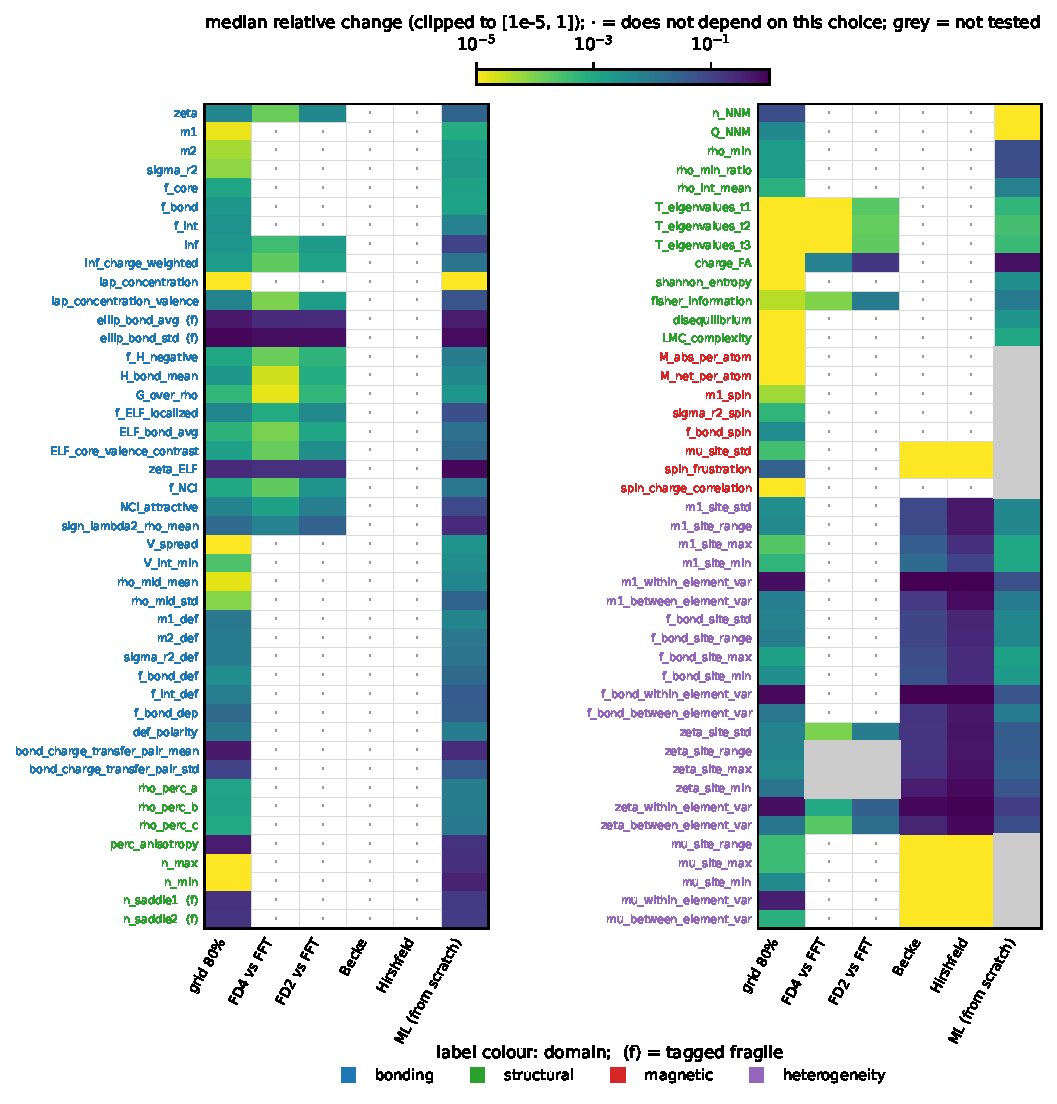
\includegraphics[width=\textwidth]{figures/fig_stability.pdf}
\caption{Stability map of the 88 descriptors of the bonding, structural,
magnetic and heterogeneity domains: median relative change when the grid is
Fourier-coarsened to 80\% of its points per axis (30 structures), when the FFT
derivatives are replaced by fourth- or second-order central differences (200
structures; 60 for the site statistics of $\zeta$), when the nearest-atom partition is replaced by Becke or
Hirshfeld weights (300 structures), and when the descriptors are computed from
a density predicted by the from-scratch ChargE3Net model instead of the DFT
density (605 test structures; Section~\ref{sec:ml}). Dots mark choices a
descriptor does not depend on; grey marks combinations not tested (the
magnetic descriptors are not available from the predicted densities). Large
values for near-zero quantities (within-element variances,
\texttt{perc\_anisotropy}, the mean pair charge transfer) reflect the small
reference value rather than an absolute error.}
\label{fig:stability}
\end{figure}

% --------------------------------------------------------------------------
\subsection{Derivatives and geometry on a periodic grid}
\label{sec:numerics:derivatives}

Gradients, Hessians and Laplacians are evaluated with the exact metric tensor,
$\nabla f=\sum_a\mathbf{b}_a\,\partial f/\partial u_a$ and
$\nabla^2 f=\sum_{ab}G_{ab}\,\partial^2 f/\partial u_a\partial u_b$ with
$G=BB^{\mathsf T}$, either as exact derivatives of the trigonometric
interpolant (FFT, the default) or by central differences of order 2--8. On 200
random structures, fourth-order differences agree with the FFT result to
about $10^{-4}$ (median) and second-order ones to 0.05--0.8\%, so the FFT
backend is the converged limit on these grids. Dropping the off-diagonal metric
terms of the Laplacian, exact only for orthogonal cells, changes the
Laplacian-based descriptors of non-orthogonal cells by a median 3--12\%. The
Laplacian-concentration ratio
$\sum_{\nabla^2\rho<0}|\nabla^2\rho_k|/\sum_k|\nabla^2\rho_k|$ of the
specification is identically $\tfrac12$ for any periodic density, since the
cell integral of $\nabla^2\rho$ vanishes (over the dataset it equals $\tfrac12$
to $9\times10^{-16}$); pydemi adds a variant restricted to the voxels outside
the core shell. Distances to the nearest nucleus come from a periodic image
search that provably contains every voxel's nearest atom, with a geometric
tie-break for equidistant images; without it, atoms on high-symmetry grid
points make the site assignment depend on round-off. The test harness checks
every descriptor for invariance under supercell expansion, translation and
rotation to $10^{-6}$.

% --------------------------------------------------------------------------
\subsection{Partition schemes}
\label{sec:numerics:partitions}

pydemi implements the nearest-atom partition (the default), a power diagram
weighted by covalent radii, Becke's fuzzy cells~\cite{becke1988} and
Hirshfeld's stockholder weights~\cite{hirshfeld1977}. In a periodic solid
Becke's product of switching functions converges only algebraically with the
number of atom images retained; pydemi truncates it at 60 images, leaving a
maximum weight error of $1.5\times10^{-2}$ in FeNi$_3$, while the Hirshfeld
weights form a partition of unity to $10^{-15}$. The whole-cell descriptors do
not depend on the partition: over 300 random structures 63 of the 88
descriptors are identical under all four. The other 25, the site statistics and
site magnetic moments, are properties of the density \emph{and} the partition.
Becke cells, which like the nearest-atom partition ignore atomic size, keep the
ranking of structures (Spearman $\rho_s\geq0.97$ for the site standard
deviations); the power diagram and Hirshfeld weights, which give larger atoms
larger regions, reorder them ($\rho_s$ down to 0.35), whereas the spread of
the site magnetic moments changes by only 1--2\%. The partition is recorded in
the metadata of every row.

% --------------------------------------------------------------------------
\subsection{Projector-augmented-wave pseudo-densities}
\label{sec:numerics:paw}

A VASP \texttt{CHGCAR} holds the pseudo-valence density plus the compensation
charge of the projector-augmented-wave (PAW) method~\cite{blochl1994,kresse1999},
which is pseudized inside each augmentation sphere of radius $R_{\mathrm{PAW}}$.
The spheres fill a median 48\% of the cell but hold most of what several
descriptor families sum over (Fig.~\ref{fig:paw}a): 86\% of $\sum|\nabla\rho|$,
the denominator of the gradient anisotropy; 87\% of the deformation density
$\int|\Delta\rho|$; and 95\% of the magnetization $\int|m|$. Four consequences
shape pydemi's definitions; the variants that exclude the spheres form an
extension, \texttt{paw}, that is off by default, so that the default
descriptor set is the same for every input.

First, the pseudo-density is negative somewhere in 61\% of the densities, and
the density minimum lies at a nucleus in two thirds of them
(Fig.~\ref{fig:paw}b), so the density floor $\rho_{\min}/\langle\rho\rangle$ is
set by the pseudization. The interstitial floor, taken outside the spheres, is
negative for only 3 structures and only weakly related to the whole-cell value
(Spearman 0.36; Fig.~\ref{fig:paw}c). Second, a pseudized atom need not have a density maximum
at its nucleus: in CaSi$_3$Pt the Si valence density forms eight lobes 0.81 and
0.83\,\AA{} from the nucleus that a fixed 0.8\,\AA{} cutoff counts as
non-nuclear maxima. Counting a maximum as non-nuclear only beyond
$\max(0.8\,\text{\AA},R_{\mathrm{PAW}})$ reduces the structures with such maxima
from 2,264 to 346. Third, the free-atom reference of the deformation density
must contain only the ZVAL valence electrons but keeps their all-electron shape
inside the spheres, so the whole-cell deformation descriptors mostly measure
the pseudization; outside the spheres (a median 54\% of the cell) they follow
chemistry, and with \texttt{AECCAR0} and \texttt{AECCAR2} pydemi uses the
all-electron density against the frozen core plus the free-atom valence
densities. Fourth, the valence counts must match the PAW datasets of the
calculation. A rule based on the electron configuration disagrees with the
datasets used for 43 of the 87 elements, which puts the reference off by up to
80 electrons per cell; pydemi reads ZVAL from the \texttt{POTCAR} or
\texttt{OUTCAR}, accepts a per-element table otherwise, falls back on a
corrected rule that reproduces 78 of the 87 elements, and records the origin of
the counts. The percolation bottlenecks, by contrast, lie at a median
$0.99\,R_{\mathrm{PAW}}$ from the nearest nucleus (Fig.~\ref{fig:paw}b), where
pseudo and all-electron densities nearly agree.

\begin{figure}[htbp]
\centering
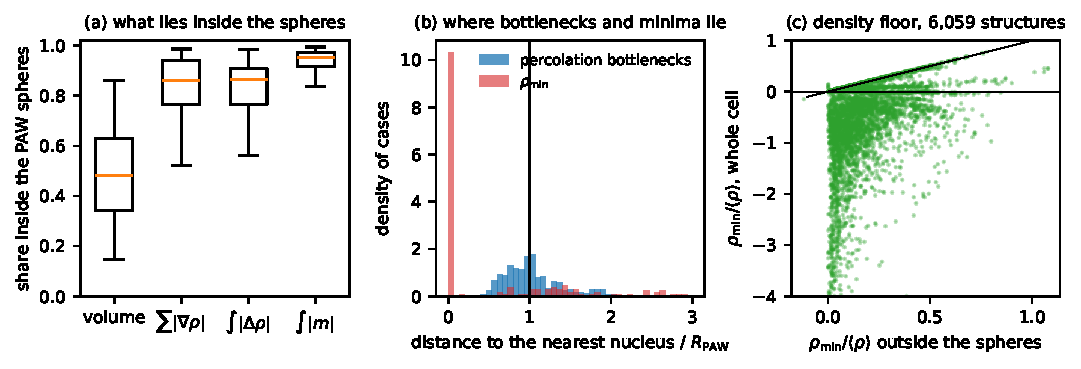
\includegraphics[width=\textwidth]{figures/fig_paw.pdf}
\caption{PAW pseudo-densities. (a) Share inside the augmentation spheres of the
cell volume, of $\sum|\nabla\rho|$, of the deformation density (100 random
structures each) and of the magnetization (150 random magnetic structures).
(b) Distance from the nearest nucleus, in units of its $R_{\mathrm{PAW}}$, of
the density minimum and of the percolation bottlenecks (200 random
structures). (c) Density floor over the whole cell against the floor outside
the spheres for all 6,059 structures.}
\label{fig:paw}
\end{figure}

% --------------------------------------------------------------------------
\subsection{The critical-point census}
\label{sec:numerics:census}

pydemi counts critical points by comparison on the grid: maxima and minima
against the 26 neighbours, saddles from the connected components of the lower
and upper link on the 14-neighbour Freudenthal triangulation~\cite{freudenthal1942},
whose link, unlike the 26-neighbour shell, is a triangulated sphere. A census
taken entirely on the Freudenthal link satisfies the Morse relation of the
three-torus for any sampled function~\cite{banchoff1970}, so the alternating
sum that pydemi reports as \texttt{euler\_consistency} is exactly
\begin{equation}
e = \big(n_{\max}^{(26)}-n_{\max}^{(14)}\big) - \big(n_{\min}^{(26)}-n_{\min}^{(14)}\big),
\end{equation}
the number of extrema whose status depends on the neighbourhood. It vanishes
for only 9.1\% of the 6,059 structures (median magnitude 5\% of all critical
points), and the mismatches follow the PAW artefacts and the low-amplitude
ripple of nearly-free-electron densities rather than the grid spacing. The
maxima and minima counts are stable, but the saddle counts change by a median
17--20\% on a coarsened grid and are tagged as fragile; the charge in the
basins of non-nuclear maxima and the percolation levels, which pydemi defines
as the highest level whose super-level set winds around the cell (detected by a
union--find over periodic images), are the stable topological descriptors.

% --------------------------------------------------------------------------
\subsection{Grid convergence and stability tags}
\label{sec:numerics:convergence}

pydemi recomputes the descriptors on a Fourier-coarsened copy of the grid to
test whether the grid resolves them. For 30 random structures, 44\% of the 88
descriptors change by at most 0.1\% (median) at 80\% of the points per axis,
and 83\% by at most 1\% (Fig.~\ref{fig:stability}). The large changes fall into
three classes: quantities that are near zero by symmetry, such as the
percolation anisotropy of cubic cells, which should be judged by absolute
error; the within-element site variances, which are numerical noise (median
$2\times10^{-9}$\,\AA$^2$ for $m_1$) in the 3,721 structures whose sites of each
element are all equivalent; and genuinely unconverged quantities, the saddle
counts and the bond ellipticity. The voxel-averaged ellipticity
$\epsilon=\lambda_1/\lambda_2-1$ of the specification diverges as
$\lambda_2\to0^-$ at bond-shell voxels away from the bond paths, and its mean
and standard deviation change by 20--70\% between any two numerical choices;
the bounded form $\epsilon/(1+\epsilon)$ changes by 0.2--1.1\% and preserves the
ranking of structures. pydemi keeps every descriptor of the specification in
its default output but tags the four unconverged ones (the two ellipticity
statistics and the two saddle counts) as fragile, provides the model-ready set
without them in one call, and offers the bounded ellipticity in an
off-by-default extension. Table~\ref{tab:corrections} lists the definitions in
which pydemi departs from, or completes, the specification.

\begin{table}[htbp]
\centering
\caption{Documented corrections to the descriptor specification, each backed by
a test or by the dataset analysis (Supporting Information, Section~S2).}
\label{tab:corrections}
\small
\begin{tabular}{p{4.2cm}p{10.3cm}}
\toprule
Item & Correction \\
\midrule
Laplacian concentration & identically $\tfrac12$ on a periodic grid; kept, plus a variant outside the core shell \\
Percolation level & the highest spanning level (the lowest is always $\min\rho$); spanning by winding around the cell, not by face contact, which would depend on the cell origin \\
All-electron reference & \texttt{AECCAR0} is the frozen core: the promolecule is \texttt{AECCAR0} plus free-atom valence densities \\
Hirshfeld charges & $Z_i=\mathrm{ZVAL}_i$ for pseudo-densities, so that the charges sum to zero \\
Valence counts & read from the calculation; fallback rule excluding the $p$-block $d^{10}$ shell and including the lanthanide and actinide semicore \\
Within-element variance & weighted by the site fraction of each element, which makes the variance decomposition exact \\
Ellipticity, saddle counts & tagged fragile; bounded ellipticity as a converged alternative \\
\bottomrule
\end{tabular}
\end{table}

\section{Validation}
\label{sec:validation}

pydemi is tested by 876 automated tests (Table~\ref{tab:validation}). Most of
them, 700, form an invariance harness that is parametrized over the registry:
every descriptor, including the extensions, is computed for a low-symmetry,
magnetic model crystal and for its $2\times2\times2$ supercell, a translation of
the origin and a rigid rotation, and must agree to $10^{-6}$ relative, so that
descriptors added later are checked automatically. The remaining tests compare
with closed forms for Slater and Gaussian densities, exact identities and
reference implementations. Beyond the test suite, each descriptor family was
checked against model densities with known answers in the course of the
dataset analysis (Supporting Information, Section~S3): 245 such checks agree
with the exact values to the round-off of the method used, or, where voxels
straddle a sharp shell boundary or a saddle falls between grid points, to a few
$10^{-3}$ (Fig.~\ref{fig:validation}).

\begin{table}[htbp]
\centering
\caption{Validation checks of the test suite and the accuracy required.}
\label{tab:validation}
\small
\begin{tabular}{p{4.5cm}p{7.3cm}r}
\toprule
Check & Content & Tolerance \\
\midrule
Invariance harness (700 tests) & every descriptor under a $2\times2\times2$ supercell, a translation and a rotation & $10^{-6}$ rel. \\
Derivatives & FFT exact for band-limited functions in a triclinic cell; FD convergence order; Hessian trace = Laplacian & $10^{-9}$--$10^{-10}$ \\
Geometry & nearest-image distances against brute force, including an extreme shear & $10^{-12}$\,\AA \\
Closed forms & radial moments of Slater densities; percolation of a simple cubic lattice at the midpoint density; uniform-gas limits of the energy densities and ELF & $10^{-2}$--$10^{-12}$ \\
Exact identities & variance decomposition; site moments sum to the net moment; partitions of unity; charge conservation; Laplacian concentration $=\tfrac12$ & $10^{-10}$--$10^{-12}$ \\
Deformation density & reference atoms equal to the crystal atoms give $\Delta\rho=0$; tabulated atoms hold ZVAL electrons & $2\times10^{-3}$ \\
Input/output & CHGCAR layouts (1, 2, 4 blocks, VASP 4/5), volume scaling, cube and XSF round trips, unit conversion & exact \\
Reference implementations & compositional descriptors against matminer; float32 mode against float64 & exact / reported \\
Sentinels and schema & no bare NaN for degenerate inputs; fixed output schema in batch mode & -- \\
Regressions & option-dependent caches, radius-scaled shells & -- \\
\bottomrule
\end{tabular}
\end{table}

\begin{figure}[htbp]
\centering
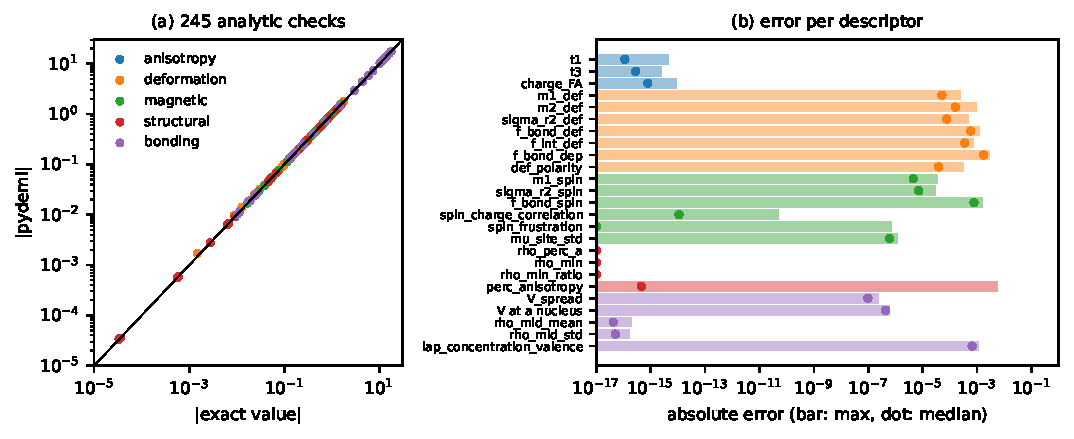
\includegraphics[width=\textwidth]{figures/fig_validation.pdf}
\caption{Analytic checks of the descriptor families on model densities with
known answers (anisotropic Gaussians, a breathing atom, bond-charge and
magnetic-sublattice models, cubic and tetragonal lattices, a rock-salt charge
transfer): (a) pydemi against the exact value, (b) median and maximum absolute
error per descriptor. The largest errors, a few $10^{-3}$, occur where voxels
straddle a sharp shell boundary or a saddle point falls between grid points.}
\label{fig:validation}
\end{figure}

\section{Application to a 6,059-structure DFT dataset}
\label{sec:application}

The dataset comprises 6,059 VASP charge densities of 87 elements: 86
elemental solids, 3,195 intermetallics and 2,778 compounds with
electronegative elements (354 borides and carbides, 80 hydrides, 653
pnictides, 548 chalcogenides, 607 oxides and 536 halides). The 4,901 runs that
include their OUTCAR share one protocol (Supporting Information,
Table~S11): single-point PBE calculations with one PAW dataset per element, a
500\,eV plane-wave cutoff, collinear spin polarization, the tetrahedron
method with Bl\"ochl corrections and an automatic $k$-mesh with a spacing of
at most about 0.1\,\AA$^{-1}$; 4.5\% of them stopped at the maximum number of
electronic steps before reaching the $10^{-6}$\,eV criterion. The remaining
1,158 runs provide only the CHGCAR. No AECCAR or LOCPOT files are included and
an ELFCAR only for 86 runs, so every descriptor below is computed from the PAW
pseudo-density, with the electron localization function reconstructed from it
for all structures alike and the electronic Hartree potential obtained by
Fourier transform.

\begin{figure}[htbp]
\centering
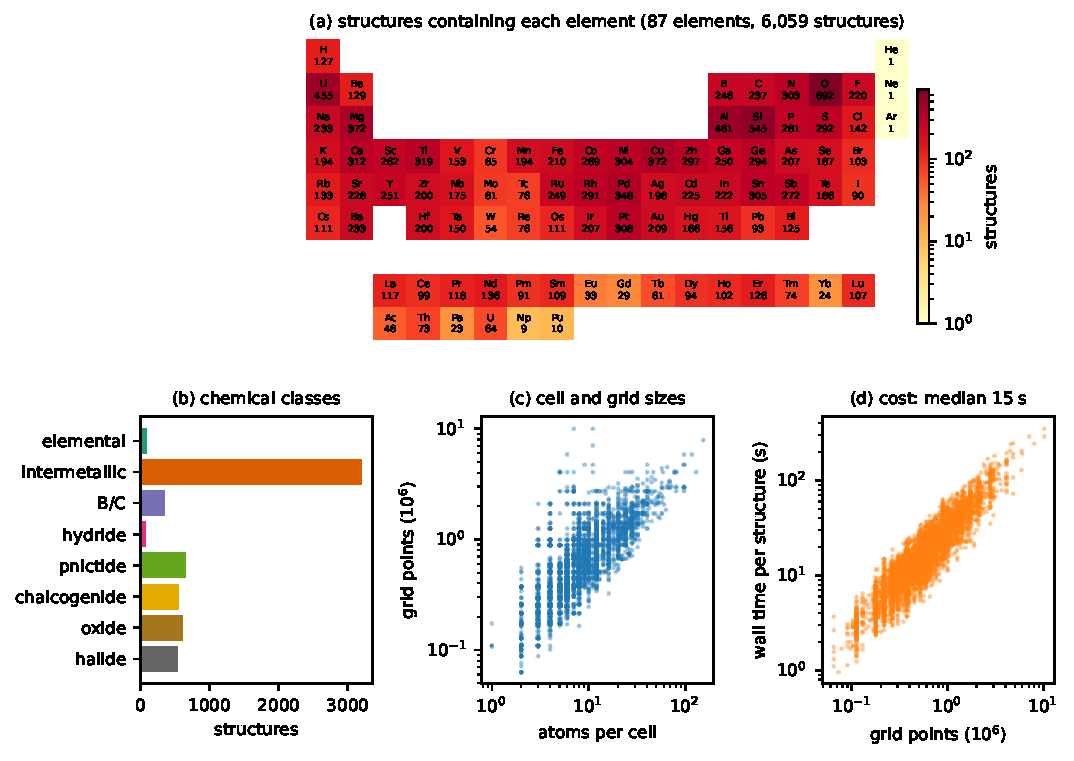
\includegraphics[width=\textwidth]{figures/fig_dataset.pdf}
\caption{The 6,059-structure dataset: (a) number of structures containing each
element, (b) chemical classes, assigned by the anions present, (c) atoms per
cell and grid points, (d) wall time of the full featurization per structure
(one worker, all domains).}
\label{fig:dataset}
\end{figure}

The cells contain 1--152 atoms (median 6) on grids of $1.8\times10^5$ to
$1.7\times10^6$ points (5th--95th percentile; Fig.~\ref{fig:dataset}). pydemi
computed all descriptors of the five domains for every structure without a
single failure, in 105 minutes on 24 worker processes (58 structures per
minute, 36.6 CPU hours in total). The median cost is 15\,s per structure and
grows linearly with the number of grid points (log--log slope 1.04), so the
cost is set by the grid rather than by the number of atoms.

The descriptors separate the chemical classes in ways that composition alone
does not (Fig.~\ref{fig:classes}). Outside the augmentation spheres, compounds
with anions put almost all of their bonding charge accumulation in the bond
shell (median share of the deformation charge 0.91--1.00), whereas elemental
solids and intermetallics put about half of it in the interstitial region
(Fig.~\ref{fig:classes}a). The interstitial density floor falls from 0.21--0.23
of the mean density for elemental solids and intermetallics to 0.02 for
halides, and follows the electronegativity difference (Spearman $-0.61$;
Fig.~\ref{fig:classes}b). The fractional anisotropy of the gradient tensor is
at the numerical floor for the non-magnetic cubic structures and exceeds $10^{-3}$ for most
structures of lower symmetry, with layered and linear-unit structures at the
top (Fig.~\ref{fig:classes}c). The percolation levels rank covalent
frameworks (borides and carbides) highest and ionic halides lowest
(Fig.~\ref{fig:classes}d). Across the 87 non-constant descriptors of the
bonding, structural, magnetic and heterogeneity domains, the largest rank
correlation of each with any of the 132 Magpie composition features has a
median of 0.44, and only one descriptor, the mean interstitial density,
exceeds 0.8 (Fig.~\ref{fig:classes}e): the density-derived descriptors carry
information that compositional featurizations do not. Section~S3 of the
Supporting Information analyses each family on the dataset in detail.

\begin{figure}[htbp]
\centering
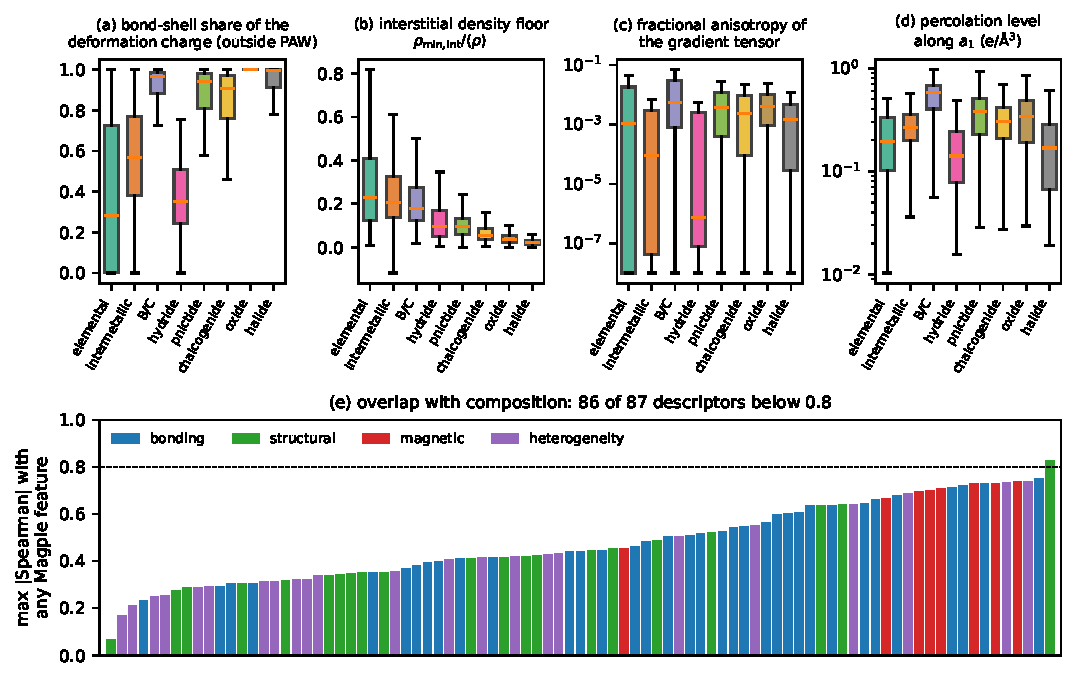
\includegraphics[width=\textwidth]{figures/fig_classes.pdf}
\caption{Descriptors across the chemical classes of the dataset: (a) bond-shell
share of the deformation charge outside the augmentation spheres
(\texttt{paw} extension), (b) interstitial density floor relative to the mean
density, (c) fractional anisotropy of the gradient tensor, (d) percolation
level along the first lattice vector (boxes: quartiles; whiskers: 1.5
interquartile ranges). (e) For each non-constant descriptor of the four
density-based domains, the largest absolute Spearman correlation with any of
the 132 Magpie composition features over the 6,059 structures.}
\label{fig:classes}
\end{figure}

% - TODO: property-prediction results, if they are to be included (targets to
%   be decided with the dataset owner).

\section{Machine-learning input path}
\label{sec:ml}
% TODO: CIF -> predicted CHGCAR model, integration into pydemi, and a
% DFT-vs-ML comparison of descriptors (to be written when available).

\section{Software availability}
% - Installation, Python API, command line, batch processing, license,
%   repository URL (TODO).

\section{Conclusions}

\section*{Acknowledgements}
% TODO

\bibliographystyle{unsrt}
\bibliography{references}

\end{document}
